% Chapter 1
\chapter{Introduction} % Write in your own chapter title
%\label{fig:INTRODUCTION}
%\lhead{CHAPTER 1. \emph{INTRODUCTION}} % Write in your own chapter title to set the page header

\section{Introduction to Data Mining}
Modern computers have made it so that every field of study is generating data at an unprecedented rate. Computers can process data in ways and speeds humans could never achieve. Data mining is the process of applying a computer-based methodology for developing knowledge from data.\par \noindent
Data mining is an interdisciplinary subfield of computer science and is the computing process of discovering patterns in large data sets involving methods at the intersection of machine learning, statistics, and database systems. The overall goal of the data mining process is to extract information from a data set and transform it into an understandable structure for further use. It involves database and data management aspects, data pre-processing, model and inference considerations, interestingness metrics, complexity considerations, post-processing of discovered structures, visualization, and online updating. Data mining is the analysis step of the ``knowledge discovery in databases" process, or KDD as depicted in Figure 1.1.
\begin{figure}[h]
\centering 
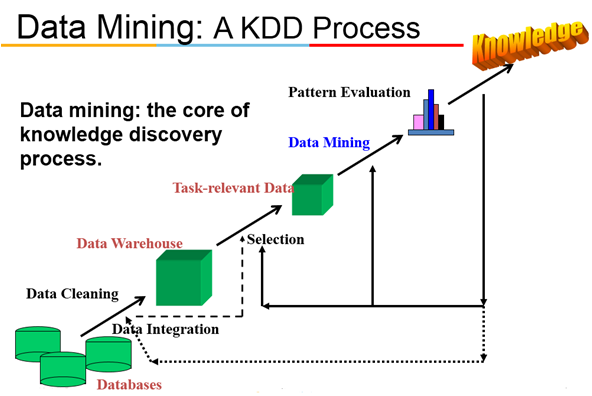
\includegraphics[scale=1.2]{kdd.png}
\caption{\label{fig:subBDDs1}Overview of steps in KDD process}
\end{figure}
\pagebreak
\section{Data Mining in Healthcare}
In today's world, healthcare information systems are capturing data in databases for research and analysis in order to assist in medical decisions. However, the data being stored is increasing on a daily basis and the data available today is in zillions and not in millions. Therefore, the process of extracting useful information is becoming difficult but data mining holds great potential for the healthcare industry to enable health systems to systematically use data and analytics to identify inefficiencies and best practices that improve care and reduce costs. Some experts believe the opportunities to improve care and reduce costs concurrently could apply to as much as 30\% of overall healthcare spending. By performing data analysis clinicians and medical researchers should be able to diagnose the disease and also assist medical science in the development of curative medicines.
\section{Introduction to Diabetes}
Recently it is observed that the number of people suffering from Diabetes Mellitus (DM), commonly referred to as diabetes, is increasing at an alarming rate and unfortunately, it is observed that a lot of young children suffer from diabetes. Diabetes is a group of metabolic disorders in which there are high blood sugar levels over a prolonged period. Symptoms of high blood sugar include frequent urination, increased thirst, and increased hunger. If left untreated, diabetes may lead to a lot of complications. Acute complications include diabetic ketoacidosis, hyperosmolar hyperglycemic state, or death. Serious long-term complications include cardiovascular disease, stroke, chronic kidney disease, foot ulcers, and damage to the eyes. Diabetes is due to either the pancreas not producing enough insulin or the cells of the body not responding properly to the insulin produced. There are three main types of diabetes mellitus:
\begin{itemize}
\item \textbf{Type 1} results from the pancreas's failure to produce enough insulin. This form was previously referred to as insulin-dependent diabetes mellitus (IDDM) or ``juvenile diabetes". The cause is unknown.
\item \textbf{Type 2} begins with insulin resistance, a condition in which cells fail to respond to insulin properly. As the disease progresses a lack of insulin may also develop. This form was previously referred to as non insulin-dependent diabetes mellitus (NIDDM) or adult-onset diabetes. The most common cause is excessive body weight and not enough exercise. 
\item \textbf{Gestational diabetes} is the third main form and occurs when pregnant women without a previous history of diabetes develop high blood sugar levels.
\end{itemize}
\par\noindent
Prevention and treatment involve maintaining a healthy diet, regular physical exercise, a normal body weight, and avoiding use of tobacco. Control of blood pressure and maintaining proper foot care are important for people with the disease. Type 1 must be managed with insulin injections. Type 2 may be treated with medications with or without insulin. Insulin and some oral medications can cause low blood sugar. Gestational diabetes usually resolves after the birth of the baby.\par\noindent
\section{Dataset}
The dataset used in this study is “The Pima Indians Diabetes Data Set” which was taken from the UCI Machine Learning Repository. The original owner of this data set is the National Institute of Diabetes and Digestive and Kidney Diseases. One major constraint placed on this dataset is that all patients selected are females at least 21 years old of Pima Indian heritage. In this project we will be building 4 classification models namely ANN, ID3, CART and C4.5.\par \noindent
The following are the parameters considered in this dataset and a brief detail pertaining to it.
\begin{itemize}
\item \textbf{Pregnancies:} Number of times pregnant
\item \textbf{Glucose:} Plasma glucose concentration- 2 hours in an oral glucose tolerance test
\item \textbf{BloodPressure:} Diastolic blood pressure (mm Hg). It indicates the pressure in the arteries when the heart rests between beats.
\item \textbf{SkinThickness:} Triceps skin fold thickness (mm). A value used to estimate body fat, measured on the right arm halfway between the olecranon process of the elbow and the acromial process of the scapula.
\item \textbf{Insulin:} 2-Hour serum insulin (mu U/ml)
\item \textbf{BMI:} Body mass index (weight in kg/(height in m)\^2)
\item \textbf{DiabetesPedigreeFunction (DPF):} DPF provides some data on diabetes mellitus history in relatives and the genetic relationship of those relatives to the patient. This measure of genetic influence gives an idea of the hereditary risk one might have with the onset of diabetes mellitus.
\item \textbf{Age:} Age (years)
\item \textbf{Outcome:} Class variable (0 or 1)
\end{itemize}
The summary statistics of the dataset attributes is tabulated in Table 1.1.
\pagebreak
\begin{table}[h]
\begin{center}
\begin{tabular}{| c | c | c | c | c | c |}
  \hline
  \textbf{Attribute} & \textbf{Type} & \textbf{Mean} & \textbf{Std} & \textbf{Min} & \textbf{Max} \\[2.5ex]
  \hline

  Pregnancy & Quantitative Discrete & 3.845 & 3.37 & 0 & 17  \\[2.5ex]
  \hline
  Glucose & Quantitative Continuous & 120.895 & 31.973 & 0 & 199  \\[2.5ex]
  \hline
  BP & Quantitative Continuous & 69.105 & 19.356 & 0 & 122  \\[2.5ex]
  \hline
  Skin Thickness & Quantitative Continuous & 20.536 & 15.952 & 0 & 99  \\[2.5ex]
  \hline
  Insulin & Quantitative Continuous & 79.799 & 115.244 & 0 & 846  \\[2.5ex]
  \hline
  BMI & Quantitative Continuous & 31.993 & 7.884 & 0 & 67.1  \\[2.5ex]
  \hline
  DPF & Quantitative Continuous & 0.472 & 0.331 & 0.078 & 2.42  \\[2.5ex]
  \hline
   Age & Quantitative Discrete & 33.241 & 11.76 & 21 & 81  \\[2.5ex]
  \hline 
\end{tabular}
\end{center}
\caption{\label{table:TT}Summary statistics of attributes in the dataset}
\end{table}
\section{Proposed System}
This project aims in building a model to classify if a person has  diabetes or not
using ANN and decision tree algorithms namely--ID3, C4.5, CART and compare the results obtained in both the models. Evaluation metrics like accuracy, error rate, sensitivity, specificity and precision will be calculated. The modules split-up of the proposed project is represented in Figure 1.2.
\begin{figure}[h]
%\vspace{-3.8in}
\centering %\offinterlineskip
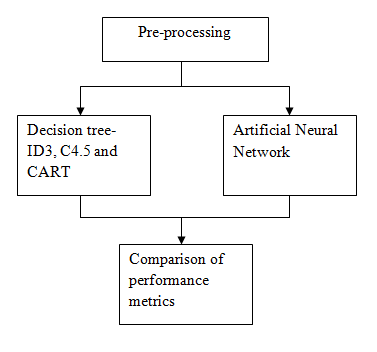
\includegraphics[scale=1.15]{modules.png}
\caption{\label{fig:subBDDs1}Modules split-up}
\end{figure}
\pagebreak
\section{Organization of the report}
In this report we start by introducing the premise of data mining, and diabetes. We then proceed to elucidate on our dataset and the proposed system. Chapter 2 covers the excerpts from our extensive literature review. The pre-processing techniques that were applied are discussed in Chapter 3 followed by the building of various classifiers. In our last chapter we summarize our results and discuss about the future scope of our above presented project.

